\documentclass[11pt, a4paper, UTF8]{ctexart}
\usepackage[body={14.64cm, 24.62cm}, centering, dvipdfm]{geometry}
\usepackage{fancyhdr}
\usepackage{listings}
\usepackage{color}
\usepackage{fontspec}
\usepackage{graphicx}
\usepackage{float}
\setmainfont{Times New Roman}

\definecolor{mygreen}{rgb}{0,0.6,0}
\definecolor{mygray}{rgb}{0.5,0.5,0.5}
\definecolor{mymauve}{rgb}{0.58,0,0.82}

\newfontface\YaHeiMono{Microsoft YaHei Mono}

\lstset{ %
  backgroundcolor=\color{white},   % choose the background color; you must add \usepackage{color} or \usepackage{xcolor}
  basicstyle=\tiny \YaHeiMono,        % the size of the fonts that are used for the code
  breakatwhitespace=true,         % sets if automatic breaks should only happen at whitespace
  breaklines=true,                 % sets automatic line breaking
  captionpos=none,                    % sets the caption-position to bottom
  commentstyle=\color{mygreen},
  morecomment=[l][\color{magenta}]{\#},    % comment style
  deletekeywords={...},            % if you want to delete keywords from the given language
  escapeinside={\%*}{*)},          % if you want to add LaTeX within your code
  extendedchars=true,              % lets you use non-ASCII characters; for 8-bits encodings only, does not work with UTF-8
  framexleftmargin=0.5em,
  frame=single,                    % adds a frame around the code
  keepspaces=true,                 % keeps spaces in text, useful for keeping indentation of code (possibly needs columns=flexible)
  keywordstyle=\color{blue},       % keyword style
  language=C++,                 % the language of the code
  otherkeywords={*,...},            % if you want to add more keywords to the set
  numbers=left,                    % where to put the line-numbers; possible values are (none, left, right)
  numbersep=1.5em,                   % how far the line-numbers are from the code
  numberstyle=\tiny\color{mygray}, % the style that is used for the line-numbers
  rulecolor=\color{black},         % if not set, the frame-color may be changed on line-breaks within not-black text (e.g. comments (green here))
  showspaces=false,                % show spaces everywhere adding particular underscores; it overrides 'showstringspaces'
  showstringspaces=false,          % underline spaces within strings only
  showtabs=false,                  % show tabs within strings adding particular underscores
  stepnumber=1,                    % the step between two line-numbers. If it's 1, each line will be numbered
  stringstyle=\color{mymauve},     % string literal style
  tabsize=4,                       % sets default tabsize to 2 spaces
  title=\lstname,                   % show the filename of files included with \lstinputlisting; also try caption instead of title
  xleftmargin=2em,xrightmargin=2em  
}


\title{可持久化本地代码仓库的实现}

\author{柯嵩宇\quad 陈乐群 \\ 2014级ACM班 \\ 上海交通大学}

\begin{document}

\maketitle
\tableofcontents
\newpage
\section{综述}
代码仓库在计算机科学的发展过程中扮演了一个非常重要的角色。一个优秀的代码仓库可以帮助程序员高效率地完成工作。这个学期的数据结构大作业,我们二人参考了git的设计编写了一个可持久化的本地代码仓库。

\section{项目简介}
\subsection{项目名称}
sit(a Simplified Git)
\subsection{支持的功能}
链式版本(即每个版本只有一个父版本)的保存与历史版本的检出以及对历史版本的修改。
\subsection{主要模块}
\begin{description}
	\item[Diff] 用于比较版本及文件间的差异。
	\item[FileSystem] 对boost::filesystem的封装,用于对文件的读写,复制及删除。
	\item[Index] 文件的索引相关的数据结构,用于保存某版本的文件的hash值。
	\item[Objects] 对版本的操作(保存文件,检出和重置版本)的数据结构的实现。
\end{description}
\subsection{主要命令}
\begin{description}
	\item[add] 把文件加入index。
	\item[checkout] 把指定的版本的文件(可以是单个文件,也可以是整个版本)复制到工作区。
	\item[commit] 将当前的index信息作为一个版本的全部文件信息并提交到仓库。
	\item[diff] 比较特定版本(全版本或特定文件)之间的差异。
	\item[init] 在当前的工作目录初始化一个版本仓库。
	\item[log] 输出已保存的版本的版本信息。
	\item[status] 输出当前工作区的文件信息。
	\item[reset] 将index或index中一个特定文件的信息重置为某个特定的版本。
	\item[rm] 将文件从index中移除。
\end{description}

\section{模块介绍}

\subsection{Color}
\subsubsection*{简介}
用于实现对输出信息的高亮,使得输出信息的可读性更佳。
\subsubsection*{实现方法}
\begin{description}
	\item[Windows] 使用Windows API实现,颜色数量较少,实际效果较差。
	\item[Unix及其他POSIX标准系统] 使用ANSI颜色序列实现,色彩丰富,实际效果较好。
\end{description}
\subsubsection*{相关文件}
Color.hpp Color.cc

\subsection{Config}
\subsubsection*{简介}
sit的配置模块,用来保存作者信息(包括作者名字和Email地址)
\subsubsection*{相关文件}
Config.hpp Config.cc
\subsection{Core}
\subsubsection*{简介}
sit的核心模块,sit的所有命令都调用Core中相关函数实现
\subsubsection*{相关文件}
Core.hpp Core.cc

\subsection{Diff}
\subsubsection*{简介}
用于比较两个文件之间或两个版本之间的差异
\subsubsection*{实现方法}
\begin{description}
	\item[版本之间] 先对两个版本的index进行diff,等到两个版本的文件列表的额差异信息(Add, Rm, Modify, Same),然后对差异信息为Modify的文件调用针对文件的比较算法。
	\item[文件之间] 对两个文件逐行Hash,对得到的Hash值列表执行LCS近似算法(时间复杂度$O(len*d)$,其中$len$为两个列表中较长的那个的值,$d$为输入数据的差异个数)。
\end{description}
\subsubsection*{相关文件}
Diff.hpp Diff.cc MurmurHash3.hpp MurmurHash3.cc

\subsection{Hash}
\subsubsection*{简介}
Hash在本项目中扮演了非常重要的角色,包括版本的管理和Diff算法的实现。
\subsubsection*{Hash在项目中的使用}
使用SHA1算法的Hash值作为文件名来保存文件。虽然效率上会受到一定的影响,但为了保证跨平台的兼容性,SHA1算法直接使用了boost库中的实现而不是git中使用了大量内嵌汇编的SHA1算法。

在针对文件的比较算法中,先使用了MurmurHash3的Hash算法,并且针对32bit和64bit的系统做出了针对性优化。

\subsection{FileSystem}
\subsubsection*{简介}
由于Windows和Linux对文件操作的API各不相同,因此使用boost库中的filesystem进行文件操作。同时为了方便代码的编写和实现一些必要的操作,对boost::filesystem进行了再封装。
\subsubsection*{主要函数}
\begin{description}
	\item[CompressCopy] 对源文件进行压缩后进行复制,主要用于add命令的实现。
	\item[CompressWrite] 将一个字符串压缩后写入文件,主要用于版本信息的压缩与写入。
	\item[DecompressCopy] 对源文件进行解压后进行复制,主要用于需要从版本库中复制文件的命令的实现。
	\item[DecompressRead] 对一个被压缩的文件使用,返回文件原来的信息,主要用于对版本信息的解压与读取。
	\item[GetRelativePath] 得到路径A相对于路径B的相对路径,用于保证在仓库的子目录中调用sit是可以得到正确的执行结果。
	\item[ListRecursive] 返回包含某一个目录下的所有文件的vector,主要用于实现需要文件夹递归的命令(add, checkout, etc)
\end{description}
\subsubsection*{相关文件}
FileSystem.hpp FileSystem.cc

\subsection{Index}
\subsubsection*{简介}
程序运行时用于处理版本的文件列表信息的数据结构,其本质是对std::unordered\_map的再封装。
\subsubsection*{实现细节}
考虑到在程序运行过程中需要处理三种类型的文件列表信息:
\begin{enumerate}
	\item 保存在".sit/index"中的已暂存的文件信息
	\item 保存在".sit/objects"中以树形结构储存的文件信息
	\item 当前工作目录的所有文件的文件信息
\end{enumerate}
其中所有的文件列表都使用<路径,SHA1~Hash值>的键值对保存。

在项目中编写了基类IndexBase,以及其针对文件中的index信息的派生类CommitIndex、针对".sit/index"中的文件信息的派生类Index、针对当前工作目录的所有文件的派生类WorkingIndex。

文件列表的读取和写入都是通过FileSystem模块来实现的。
\subsubsection*{相关文件}
Index.hpp Index.cc

\subsection{Objects}
\subsubsection*{简介}
作为文件与Index之间的中间数据结构,在Index与Commit文件的转换中具有重要的作用。tree类型的object以树形结构保存了index中的文件列表,清楚的记录了文件和路径的关系。
\subsubsection*{实现细节}
包含三种类型的Objects:
\begin{description}
	\item[commit] 这个类型的Objects表示该文件记录的是一个版本信息,包含文件的信息和该commit的信息(作者,时间,以及COMMIT\_MSG)。
	\item[tree] 表示这个文件是一个文件列表,记录了同一个文件夹下所有文件的信息,每行一个object,分别是,文件权限,该object的类型,SHA1 Hash值,以及object的名字(如果是blob类型则是文件名,如果是tree类型,则表示这个文件夹的名字)。
	\item[blob] 一个基本的object类型,表示它是路径树上的叶子节点,记录的是相应的文件(可以是文本文件,也可以是二进制文件)。
\end{description}
保存Object的结构体:
\begin{lstlisting}
struct TreeItem {
	int mode;                         // Linux文件权限,如10644
	ObjectType type;                  // 这个Object的类型:tree or blob
	std::string id;                   // 文件的SHA1值,其实等价于文件的路径
	boost::filesystem::path filename; // 文件路径
};
\end{lstlisting}
保存Commit信息的结构体
\begin{lstlisting}
struct Commit {
	std::string tree;      // 以REPO_ROOT为根的目录树的SHA1 Hash值
	std::string parent;    // 该提交的父版本
	std::string author;    // 作者的名字,Email地址,时间戳,时区
	std::string committer; // 提交者的名字,Email地址,时间戳,时区
	std::string message;   // Commit Messages
};
\end{lstlisting}
\subsubsection*{相关文件}
Objects.hpp Objects.cc

\subsection{Refs}
\subsubsection*{简介}
由于处理与版本指针相关的引用信息,如,当前工作区的版本(HEAD指针),当前分支的版本指针(指向当前分支的最后一个版本,由于目前的sit不支持分支功能,故只有一个默认生成的master分支)。该模块的目的主要是为了减少以后需要增加分支功能的时候的工作量。
\subsubsection*{相关文件}
Refs.hpp Refs.cc

\subsection{Status}
\subsubsection*{简介}
用于处理工作区和index以及版本库之间的关系,输出当前工作区的状态。
\subsubsection*{实现细节}
使用了Index模块中的WorkingIndex类,会与保存在".sit/index"中的Index以及HEAD指针指向的commit的Index比较,得出哪些文件是新出现且没有加入index的,那些文件已经被index记录,那些文件被删除。如果WorkingIndex中的所有文件记录与HEAD指向的commit的文件记录都相同那么认为工作区是Clean的。checkout操作在检出commit的时候要求工作区必须是Clean的。
\subsubsection*{相关文件}
Status.hpp Status.cc

\subsection{Util}
\subsubsection*{简介}
重要的一个模块,作为整个工程的工具模块,其中包含了对boost库中SHA1算法的封装,以及根据当前的objects目录提供的SHA1值的补全功能,增强了sit的易用性。

在这个模块里还定义了sit的异常类SitException,用于对用户的非法操作给出提示与警告。
\subsubsection*{相关文件}
Util.hpp Util.cc

%===============================================================================================
%===============================================================================================
%===============================================================================================
%===============================================================================================

\section{命令介绍}
sit使用了boost中的program\_options模块来格式化处理命令行参数。除了非默认参数外,其余参数在使用时均需要满足下列格式之一:
\begin{lstlisting}[language=sh,basicstyle=\small\YaHeiMono,numbers=none]
--<option_name>=<option_value>
-<option_abbr>=<option_value>
\end{lstlisting}

其中等号可以用空格代替。默认参数可以省略掉等号前面的部分。 

参数中commit-id都是代表某个commit的SHA1值(或版本指针(HEAD,index,work,master))。
\subsection{add}
\subsubsection* {Introduction}
把文件内容加入到index
\subsubsection*{Usage}
\begin{lstlisting}[language=sh,basicstyle=\small\YaHeiMono,numbers=none]
sit add <path_1> [<path_2> ...]
\end{lstlisting}
\subsubsection*{Options}
\begin{description}
	\item[\YaHeiMono <path>(默认参数)] 要加入index的文件(或文件夹,如果是文件夹将递归加入该文件夹下所有的子文件(夹))
\end{description}

\subsection{checkout}
\subsubsection*{Introduction}
将代码库/index中的文件解压并复制到当前的工作区中。
\subsubsection*{Usage}
checkout命令有两种基本形式:
\begin{lstlisting}[language=sh,basicstyle=\small\YaHeiMono,numbers=none]
sit chekcout [--commit=<commit-id>]
\end{lstlisting}
\begin{lstlisting}[language=sh,basicstyle=\small\YaHeiMono,numbers=none]
sit checkout [--commit=<commit-id>] --path=<path_1> [--path=<path_2> ...]
\end{lstlisting}
\subsubsection*{Options}
\begin{description}
	\item[\YaHeiMono commit] 指定复制到工作区的文件来源,接受的值为任意一个commit的ID的前缀(可以自动补全)或者是版本指针(目前支持的有HEAD,index,master),默认值为index。
	\item[\YaHeiMono path(默认参数)] 指定需要复制到工作区的文件(夹),如果没有指定任何一个文件,那么checkout将复制该commit的所有文件到工作区,并且将HEAD指针指向checkout的commit(如果commit参数为index则不改变HEAD指针)。
\end{description}

\subsection{config}
\subsubsection*{Introduction}
修改该仓库的配置,目前支持的仓库配置有用户名和用户的Email地址。
\subsubsection*{Usage}
\begin{lstlisting}[language=sh,basicstyle=\small\YaHeiMono,numbers=none]
sit config <key> <value>
\end{lstlisting}
\subsubsection*{Options}
\begin{description}
	\item[\YaHeiMono <key>] 修改配置的字段名
	\item[\YaHeiMono <value>] 新的配置值
\end{description}

\subsection{commit}
\subsubsection*{Introduction}
将当前``.sit/index''文件中所记录的index信息写入版本仓库。
\subsubsection*{Usage}
\begin{lstlisting}[language=sh,basicstyle=\small\YaHeiMono,numbers=none]
sit commit  [--amend] [--all | -a] [--message | -m COMMIT_MSG]
\end{lstlisting}
\subsubsection*{Options}
\begin{description}
	\item[\YaHeiMono all,a] 等价于在执行commit操作之前先执行一次`add <REPO\_ROOT>',其中REPO\_ROOT表示仓库的绝对路径。
	\item[\YaHeiMono amend] 表示新的commit将取代原来的HEAD所指向的commit在版本链中的位置。\\\textbf{注意:如果没有amend参数,那么commit只有当HEAD指针与master指针相等的时候才会执行(为了保证版本链的唯一)。}
	\item[\YaHeiMono message,m] 以参数的形式提供用于描述该commit改动的信息。
\end{description}

\subsection{diff}
\subsubsection*{Introduction}
比较两个commit的文件信息(或两个不同版本的同一文件(夹))的差异。
\subsubsection*{Usage}
\begin{lstlisting}[language=sh,basicstyle=\small\YaHeiMono,numbers=none]
sit diff [--base-id=<commit-id>] [--target-id=<commit-id>] [--path=<path> ...]
\end{lstlisting}
\subsubsection*{Options}
\begin{description}
	\item[\YaHeiMono base-id] 作为基准的commit的ID,默认值为index。
	\item[\YaHeiMono target-id] 比较差异的commit的ID,默认值为work(即当前的工作区)。
	\item[\YaHeiMono path(默认参数)] 用于指定需要比较的文件(夹),如果没有指定任何一个文件,那么将比较两个版本的index以及每一个有修改的文件。
\end{description}

\subsection{gc}
\subsubsection*{Introduction}
删除那些``不再需要''的object,释放它们占用的硬盘空间。
\subsubsection*{Usage}
\begin{lstlisting}[language=sh,basicstyle=\small\YaHeiMono,numbers=none]
sit gc
\end{lstlisting}

\subsection{init}
\subsubsection*{Introduction}
在当前的工作目录下建立一个sit的版本仓库,如果已经存在了一个sit的版本仓库,那么将把这个版本仓库初始化(即删除再创建)。
\subsubsection*{Usage}
\begin{lstlisting}[language=sh,basicstyle=\small\YaHeiMono,numbers=none]
sit init
\end{lstlisting}

\subsection{log}
\subsubsection*{Introduction}
以当前HEAD指针指向的commit为最后的commit,输出该commit以及它的所有父版本的信息(作者,提交时间,提交信息)。
\subsubsection*{Usage}
\begin{lstlisting}[language=sh,basicstyle=\small\YaHeiMono,numbers=none]
sit log
\end{lstlisting}

\subsection{status}
\subsubsection*{Introduction}
将当前的工作区的index和HEAD指针所指向的commit的index进行比较,输出新增的文件,修改过的文件,被删除的文件。
\subsubsection*{Usage}
\begin{lstlisting}[language=sh,basicstyle=\small\YaHeiMono,numbers=none]
sit status
\end{lstlisting}

\subsection{reset}
\subsubsection*{Introduction}
将仓库中某个commit中保存的文件信息恢复到当前的index中。
\subsubsection*{Usage}
reset命令有两种形式:
\begin{lstlisting}[language=sh,basicstyle=\small\YaHeiMono,numbers=none]
sit reset [--hard] [--commit=<commit-id>]
\end{lstlisting}
\begin{lstlisting}[language=sh,basicstyle=\small\YaHeiMono,numbers=none]
sit reset  [--commit=<commit-id>] --path=<path_1> [--path=<path_2> ...]
\end{lstlisting}

第一种形式会将当前分支的版本指针移动到指定的commit上。(移动版本链的链表尾,操作后尾后的commit还会存在仓库中,此时执行gc命令将把这些commit相关的且没有被其他文件引用的objects清理掉。)

第二种形式必须指定最少要恢复的文件,否则sit会将其解释为第一种形式。
\subsubsection*{Options}
\begin{description}
	\item[\YaHeiMono hard] 如果给出``--hard''参数,那么reset命令在恢复index中的文件信息的同时,会从仓库中复制相应的文件到工作区。如果没有则reset命令只会对index进行修改。
	\item[\YaHeiMono commit] 用于指定要恢复到index的文件信息来自于哪一个commit。
	\item[\YaHeiMono path(默认参数)] 用于指定恢复哪些文件的信息。\textbf{注意:path参数和hard参数不能同时存在。如果必要的话,可以先后执行reset和checkout两个命令来满足要求。}
\end{description}

\newpage
\section{压力测试}
从github上获取redis 2.4的版本仓库用于测试git与sit的时空效率。
\subsection{测试方法}
在redis中以master分支为基准,找出一条版本链,如果这个版本是merge得到的,那么就选择它的第一个父版本。然后将版本链上的每一个版本checkout,然后执行add和commit命令,同时监控其CPU时间的消耗。
\subsection{空间占用}
把所有的文件都add和commit到仓库中后分别查看``.sit''和``.git''文件夹的大小。
\begin{center}
\begin{tabular}{|l|r|r|}
\hline
                         & 仓库大小 & 相对大小\\
\hline
.git                     & 94324 kB           &   100\% \\
\hline
.sit(with compression)   & 82180 kB           &  87.1\% \\
\hline
.sit(without compression)& 264004 kB          & 279.9\% \\
\hline
\end{tabular}
\end{center}
\subsection{时间使用}
比较了sit(有无压缩功能)与git的时间效率(结果见后图)。
\begin{figure}[H]
	\centering
	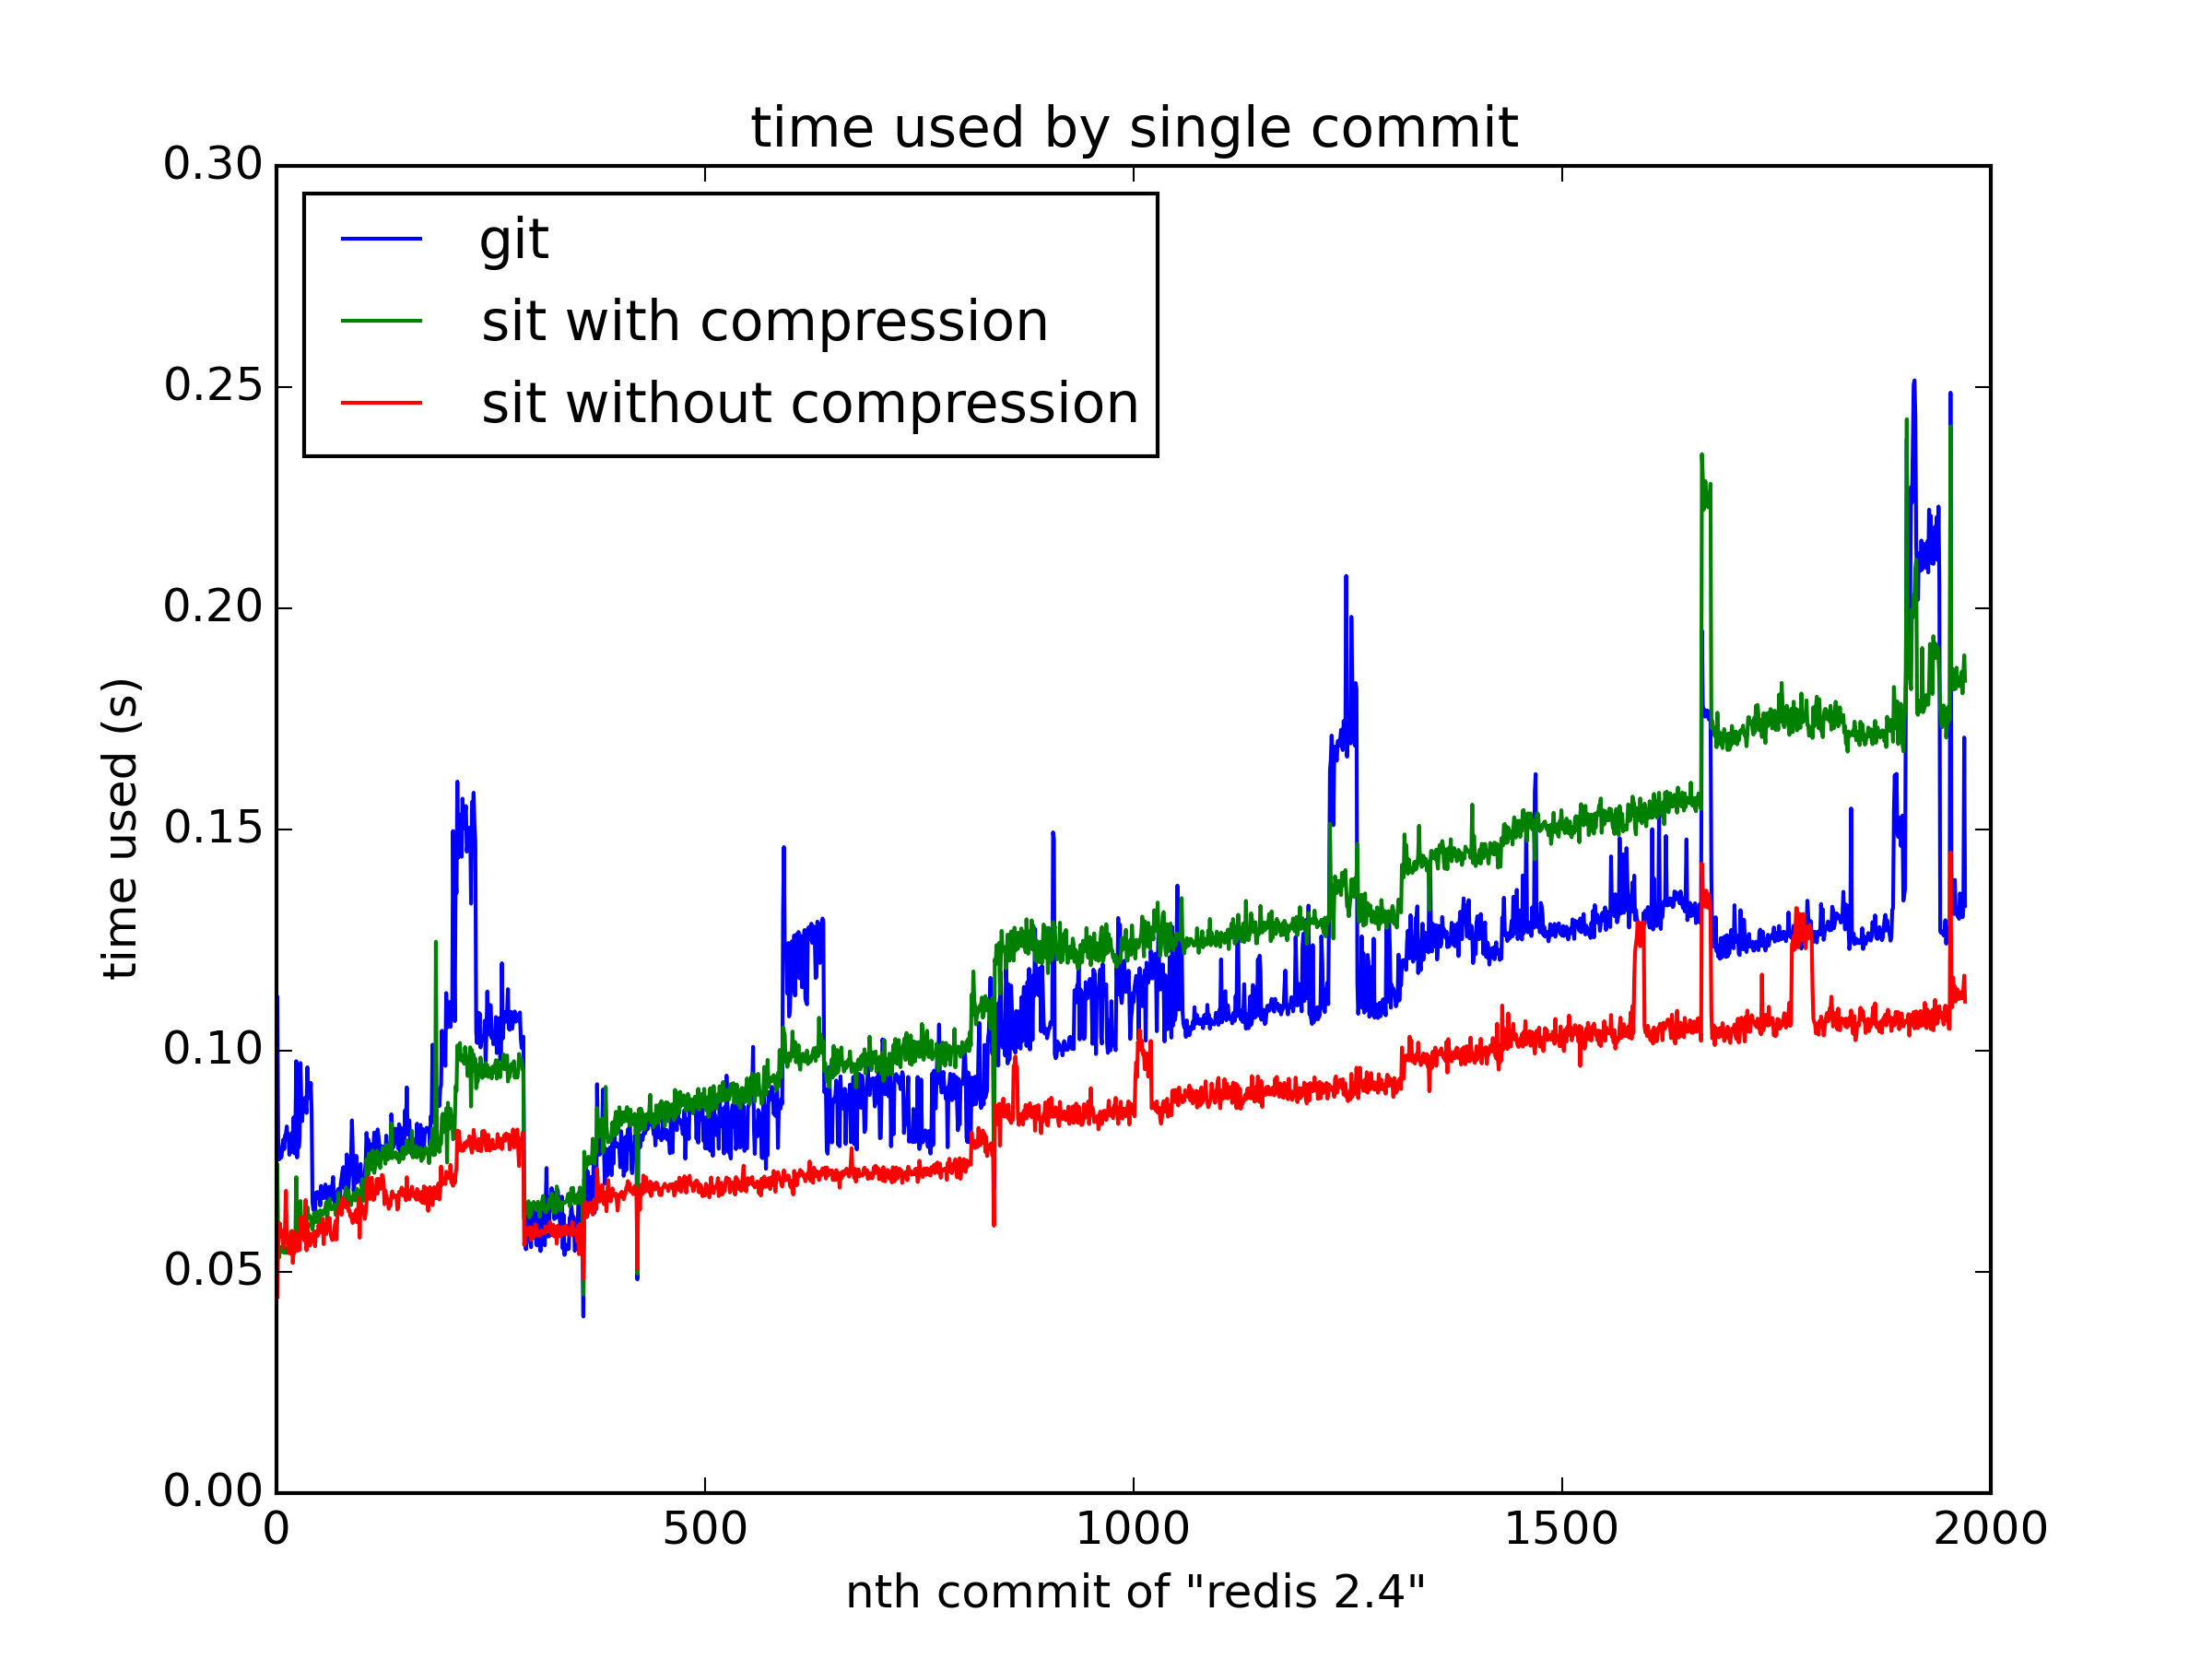
\includegraphics[scale=0.7]{figure_1.png}
	\caption{单次commit操作所需要的时间}
\end{figure}
\begin{figure}[H]
	\centering
	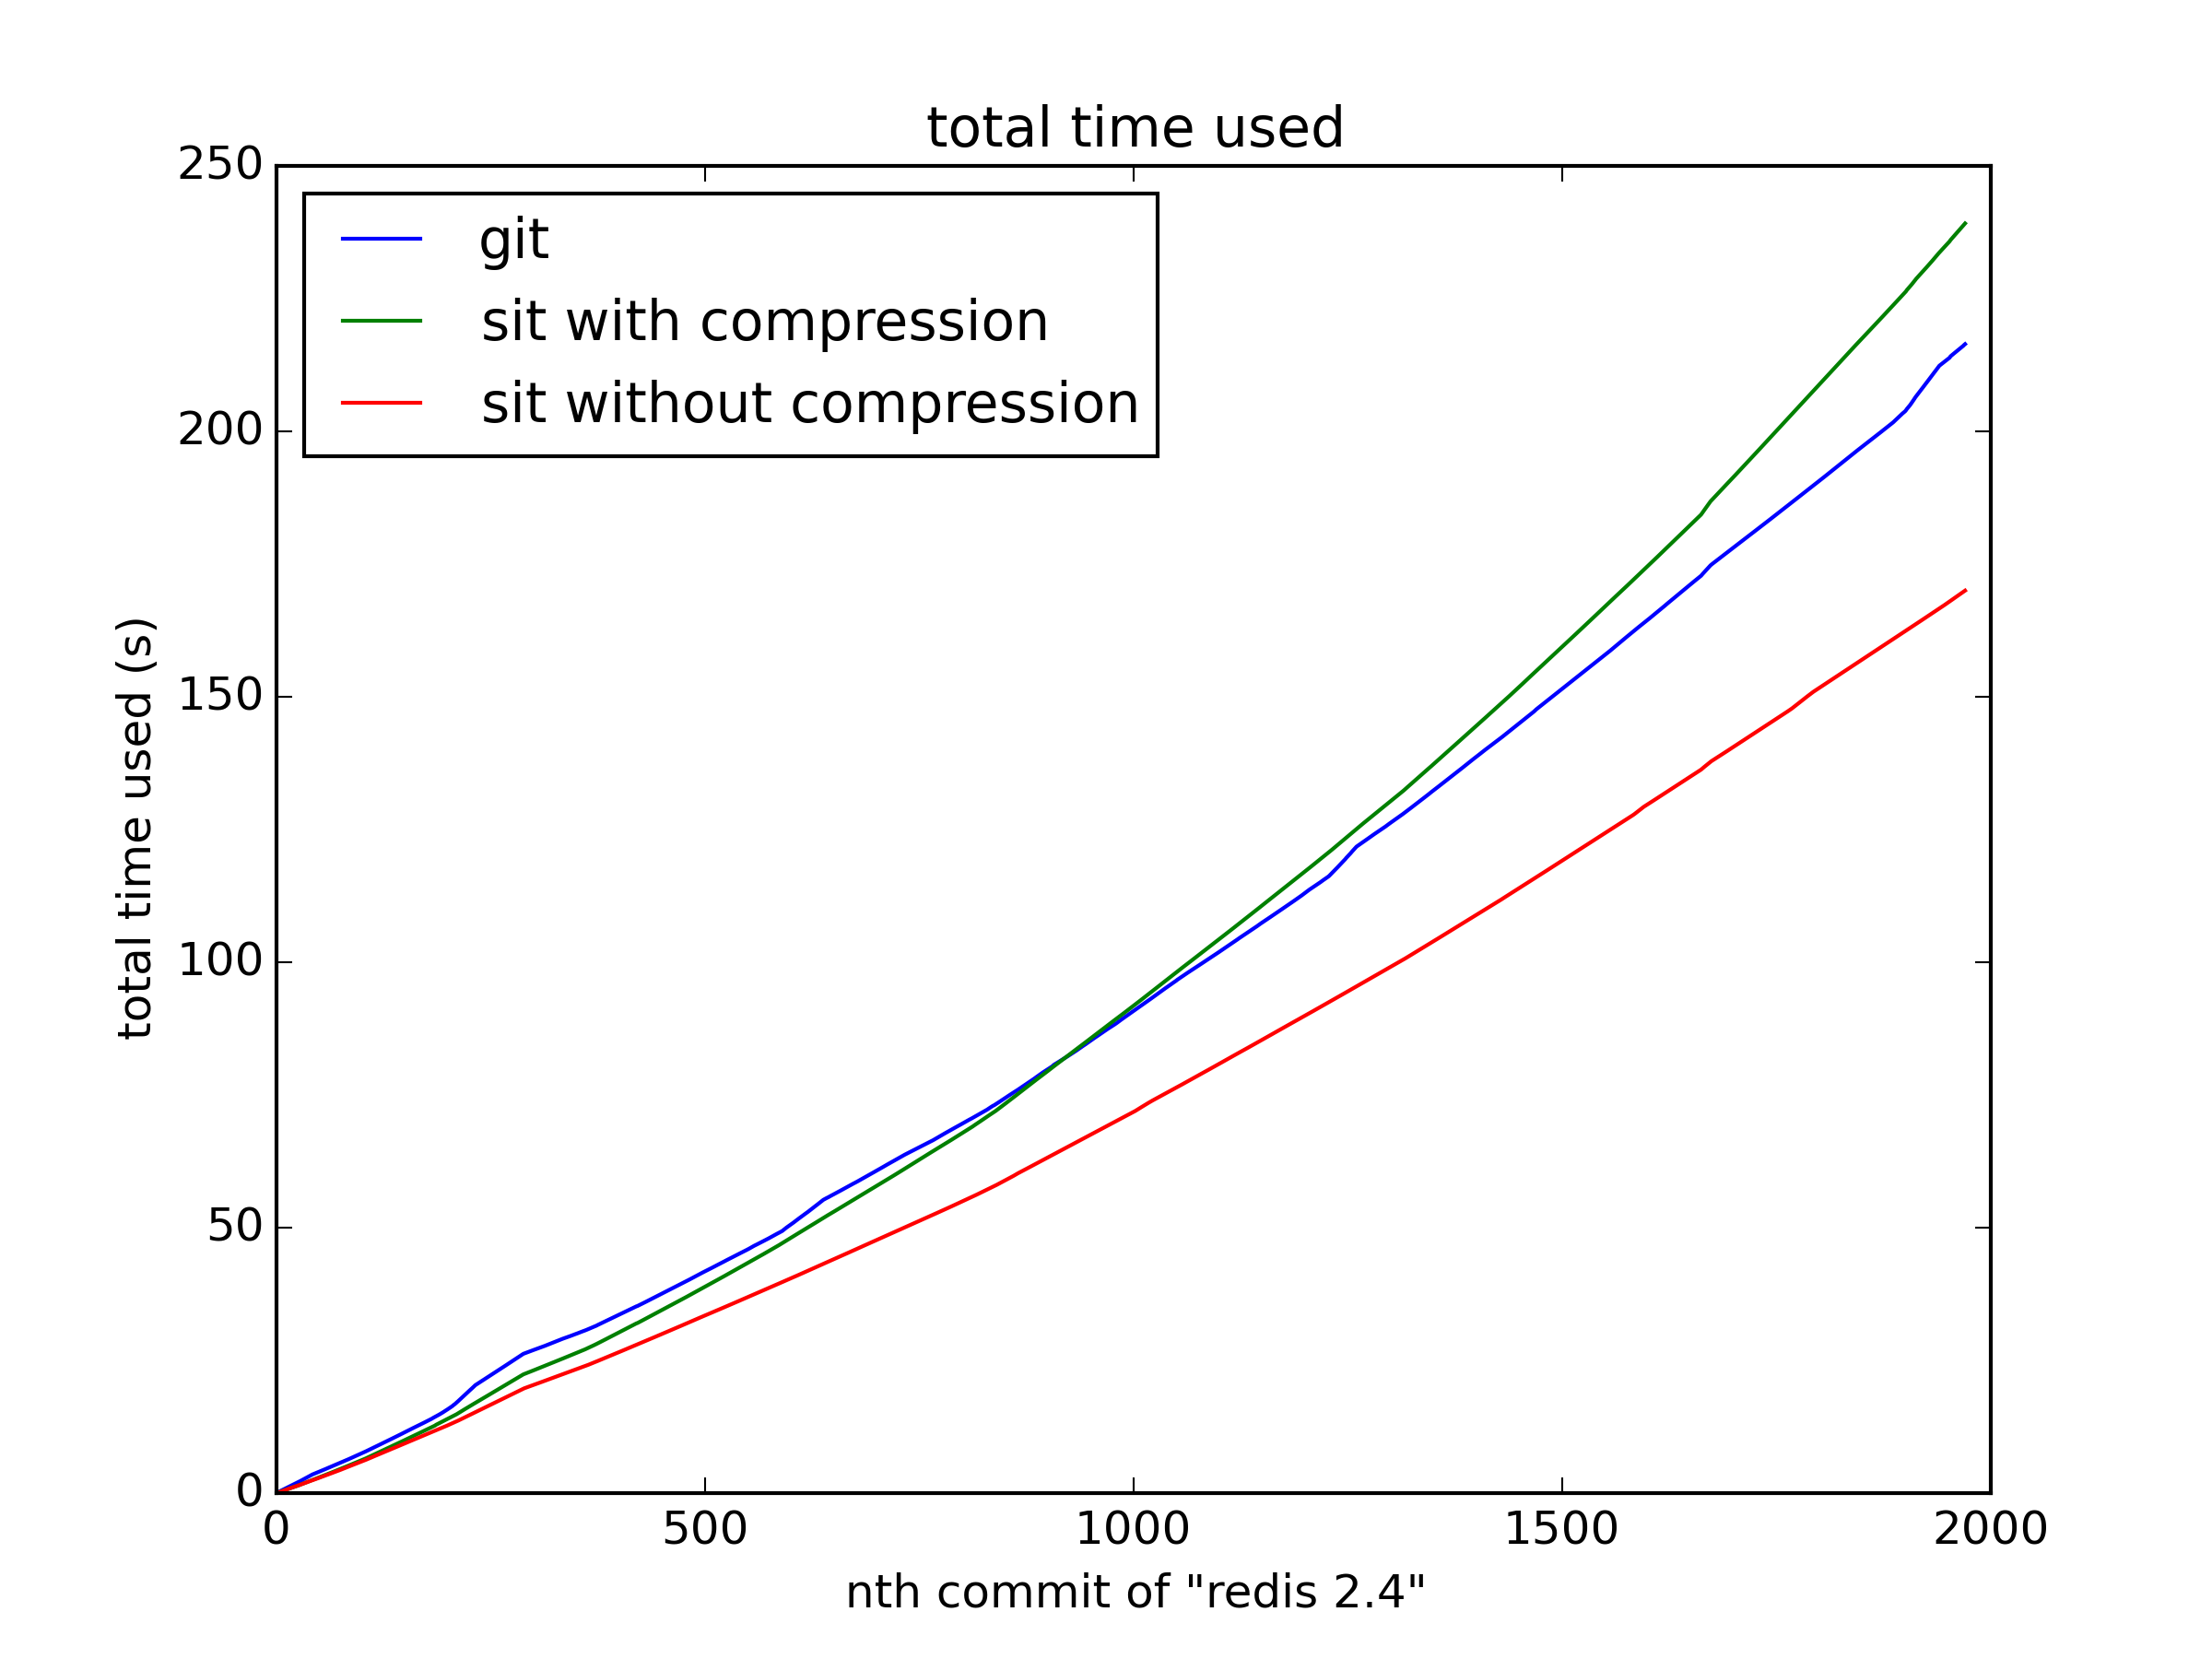
\includegraphics[scale=0.7]{figure_2.png}
	\caption{耗去的总时间}
\end{figure}
\subsection{结论}
从时间和空间的测试结果可以初步得出结论:在不支持压缩的情况下,sit比git运行的更快,当仓库占用的空间比较可怕,大约是git的2.8倍;支持压缩的sit的运行速度明显下降,相对git略慢,但是在空间效率上比git更好。

\section{总结}
在这个编写这个项目的过程中,遇到了不少的困难。考虑到用户的使用体验,我们在设计参数和处理命令的时候增加了很多人性化的设计。就目前来说sit中大量使用了C++STL中的模版来存储各类信息,同时为了保证多平台的支持,使用了boost库来实现与文件系统的交互,因此,在效率上还有一定的提升空间。当然,目前sit的功能还比较孱弱,有一些不人性化的处理还有待完善。
\end{document}